\documentclass[progressbar=head]{beamer}
\usetheme{dresden}
\usepackage[utf8]{inputenc}
\usepackage[english]{babel}
\usepackage{amsmath}
\usepackage{amsfonts}
\usepackage{amssymb}
\usepackage{graphicx}

\usepackage{ mathrsfs }

\usepackage{ bbold }

%\usepackage{cite}

\usepackage{caption}

% packages
\usepackage{mdframed}

%for links
%\usepackage{hyperref}

% for units
\usepackage{siunitx}

% for the vector on ones
\usepackage{bbm}

% to get the units correctly for printing
%\usepackage{layouts}

% for commenting multiple lines efficiently
\usepackage{comment}

% for fancy tables
\usepackage{booktabs}

%\usepackage{esint}

%\usepackage{mathtools}

% for bibliography
\usepackage[style=authoryear]{biblatex}
\addbibresource{refs.bib}

\usepackage{csquotes}

%%%%%%%%%%%%%%%%%%%%%%%%%%%%%%%%%%%%%%%%%%%%%%%%%%%%%%%%%%%%%%%%%%%%%%%%%%%%%%%%%%%%%%
%%%%%%%%%%%%%%%%%%%%%%%%%%%%%%%%%%%%%%%%%%%%%%%%%%%%%%%%%%%%%%%%%%%%%%%%%%%%%%%%%%%%%%

\title{New Methods in Electrical Source Imaging Based on EEG and Post-Mortem Pathology Data}
\date{August 7, 2024}
\author{Julio Cesar Enciso-Alva}
\institute{University   of Texas at Arlington}

%%%%%%%%%%%%%%%%%%%%%%%%%%%%%%%%%%%%%%%%%%%%%%%%%%%%%%%%%%%%%%%%%%%%%%%%%%%%%%%%%%%%%%
%%%%%%%%%%%%%%%%%%%%%%%%%%%%%%%%%%%%%%%%%%%%%%%%%%%%%%%%%%%%%%%%%%%%%%%%%%%%%%%%%%%%%%

\allowdisplaybreaks

%\definecolor{mygreen}{rgb}{0,0.6,0}
%\definecolor{mygray}{rgb}{0.5,0.5,0.5}
%\definecolor{mymauve}{rgb}{0.58,0,0.82}


%\addtocontents{toc}{\noindent\mbox{Chapter}\hfill\mbox{Page}}%

%\renewcommand{\listalgorithmname}{LIST OF ALGORITHMS}
%\addtocontents{loa}{\noindent\mbox{Algorithm}\hfill\mbox{Page}}
%\numberwithin{algorithm}{chapter}

\newcommand{\ts}{\textsuperscript}
\newcommand{\Supp }{\rm Supp}
\newcommand{\pa }{\partial }
\newcommand{\f}{\frac}
\newcommand{\me}{\mathrm{e}}
\newcommand{\mi}{\mathrm{i}}
\newcommand{\mpi}{\mathrm{\pi}}
\newcommand{\msh}{\mathrm{sinh}\,}
\newcommand{\mch}{\mathrm{cosh}\,}
\newcommand{\mth}{\mathrm{tanh}\,}

%%%%%%%%%%%%%%%%%%%%%%%%%%%%%%%%%%%%%%%%%%%%%%%%%%%%%%%%%%%%%%%%%%%%%%%%%%%%%%%%%%%%%%
%%%%%%%%%%%%%%%%%%%%%%%%%%%%%%%%%%%%%%%%%%%%%%%%%%%%%%%%%%%%%%%%%%%%%%%%%%%%%%%%%%%%%%

%% PARENTHESIS

\newcommand{\sset}[1]{ \left\{ #1 \right\} }
\newcommand{\ppar}[1]{ \left( #1 \right) }
\newcommand{\spar}[1]{ \left[ #1 \right] }

\newcommand{\abss}[1]{ \left| {#1} \right| }

\newcommand{\nnorm}[1]{\left\lVert #1 \right\rVert}

%% MATRICES

%\newcommand{\R}{\mathbb{R}}
%\newcommand{\ones}[1]{ \mathbbm{1}_{N_{#1}} \mathbbm{1}_{N_{#1}}^\intercal }

\newcommand{\ones}{\mathbbm{1}}

\newcommand{\trans}{^T}
\newcommand{\iinv}{^{-1}}
\newcommand{\pinv}{^\dagger}

\newcommand{\diag}[1]{\text{diag}\ppar{ #1 }}

%% PROBABILITY

\newcommand{\prob}{\text{Prob}}
\newcommand{\given}{\;\middle|\;}

\newcommand{\vvar}[1]{\text{Var}\ppar{#1}}
\newcommand{\ccov}[1]{\text{Cov}\ppar{#1}}

%\newcommand{\ccon}[2]{\left\phantom{(} #1 \mathrel{}\middle|\mathrel{} #2 \right\phantom{)}}

%% OPTIMIZATION

\DeclareMathOperator*{\argmax}{arg\,max}
\DeclareMathOperator*{\argmin}{arg\,min}

%% BIG LETTERS

\newcommand{\J}{\mathbf{J}}
\newcommand{\Y}{\mathbf{Y}}
\newcommand{\G}{\mathbf{G}}

\newcommand{\PA}{\mathbf{P}}
\newcommand{\SA}{\mathbf{S}}
\newcommand{\AAA}{\mathbf{A}}

\newcommand{\RA}{\mathbf{R}}
\newcommand{\BA}{\mathbf{B}}

\newcommand{\U}{\mathbf{U}}
\newcommand{\N}{\mathbf{N}}

\newcommand{\rr}{\mathbf{r}}
\newcommand{\sa}{\mathbf{s}}
\newcommand{\dd}{\mathbf{d}}

\newcommand{\ee}{\mathbf{e}}
\newcommand{\mm}{\mathbf{m}}

\newcommand{\V}{\mathbf{V}}

\newcommand{\Gbar}{\overline{\mathbf{G}}}
\newcommand{\Ybar}{\overline{\mathbf{Y}}}

%% BASICS

\newcommand{\R}{\mathbb{R}}

\newcommand{\id}{\mathbf{I}}
\newcommand{\norm}{\mathcal{N}}

%% DEPRECATED

\newcommand{\GAM}{\mathbf{\Gamma}}
\newcommand{\SIG}{\mathbf{\Sigma}}
\newcommand{\ga}{\pmb{\gamma}}

\newcommand{\jt}{\mathbf{j}}

\newcommand{\W}{\mathbf{W}}

\newcommand{\LL}{\mathbf{\Lambda}}


%%%%%%%%%%%%%%%%%%%%%%%%%%%%%%%%%%%%%%%%%%%%%%%%%%%%%%%%%%%%%%%%%%%%%%%%%%%%%%%%%%%%%%
%%%%%%%%%%%%%%%%%%%%%%%%%%%%%%%%%%%%%%%%%%%%%%%%%%%%%%%%%%%%%%%%%%%%%%%%%%%%%%%%%%%%%%

%\def\SPSB#1#2{\rlap{\textsuperscript{#1}}\SB{#2}}
%\def\SP#1{\textsuperscript{#1}}
%\def\SB#1{\textsubscript{#1}}


%%%%%%%%%%%%%%%%%%%%%%%%%%%%%%%%%%%%%%%%%%%%%%%%%%%%%%%%%%%%%%%%%%%%%%%%%%%%%%%%%%%%%%
%%%%%%%%%%%%%%%%%%%%%%%%%%%%%%%%%%%%%%%%%%%%%%%%%%%%%%%%%%%%%%%%%%%%%%%%%%%%%%%%%%%%%%

\begin{document}

\AtBeginSection[]{
  \begin{frame}
  \vfill
  \centering
  \begin{beamercolorbox}[sep=8pt,center,shadow=true,rounded=true]{title}
    \usebeamerfont{title}\insertsectionhead\par%
  \end{beamercolorbox}
  \vfill
  \end{frame}
}



{
%\metroset{background=dark}
\maketitle

\begin{frame}%{Overview}
\tableofcontents[pausesections]
\end{frame}
}

\addcontentsline{toc}{section}{Foreword}

\begin{frame}{Family}
Picture of the family and Pachuca.
\end{frame}


{
%\metroset{background=dark}
\section{Introduction}
}

\begin{frame}{Why Electrical Source Imaging}
\begin{itemize}
\item Multiple EEG patterns have been found to be related to normal and pathological states \footfullcite{niedermeyer2011niedermeyer}. 
\item Electrical Source Imaging (ESI) is a framework to locate the neural sources of electric/magnetic activity.
\item EEG has high resolution in time, low resolution in space. 
\item ESI is ill-posed, in the sense of Hadamard.
\end{itemize}
\begin{figure}
\centering
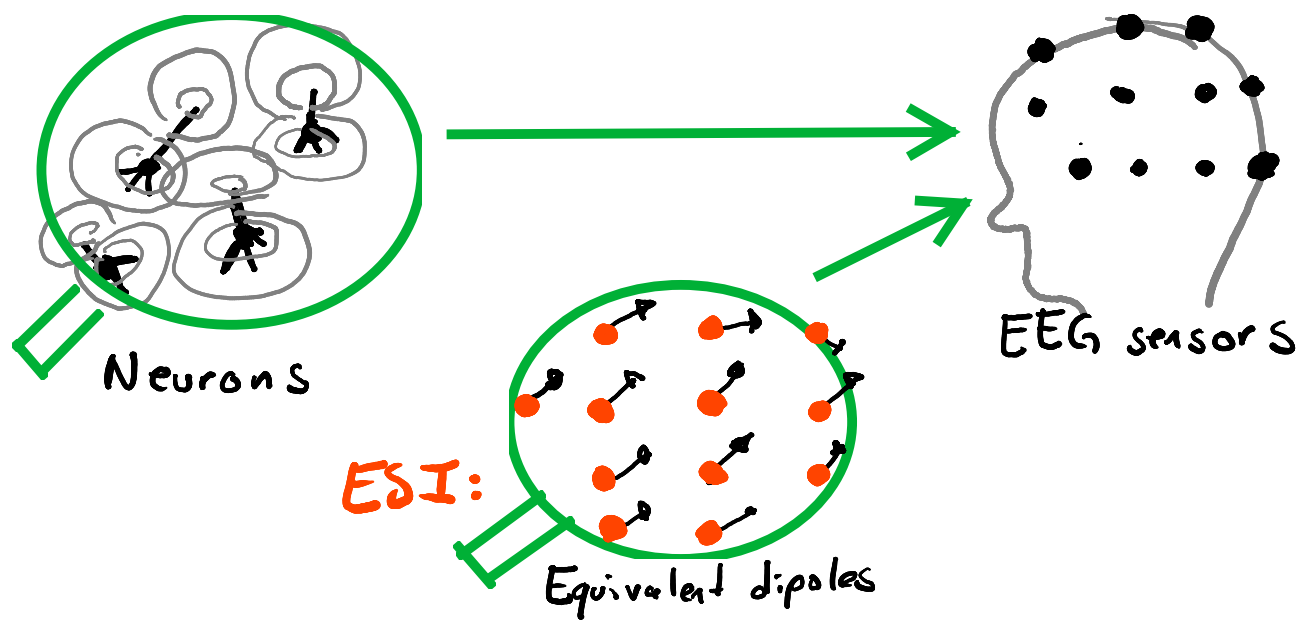
\includegraphics[width=0.6\linewidth]{./img_oldbeamer/sketch03}
\end{figure}
\end{frame}



\begin{frame}{What is Electrical Source Imaging}
%Post-synaptic potentials from neurons produces a small current density field that can be approximated by a dipole.


EEG recordings can be modeled by a system in the form 
\begin{equation}
\mathbf{Y} = \mathbf{G} \mathbf{S} + \varepsilon
\end{equation}

\begin{figure}
\centering
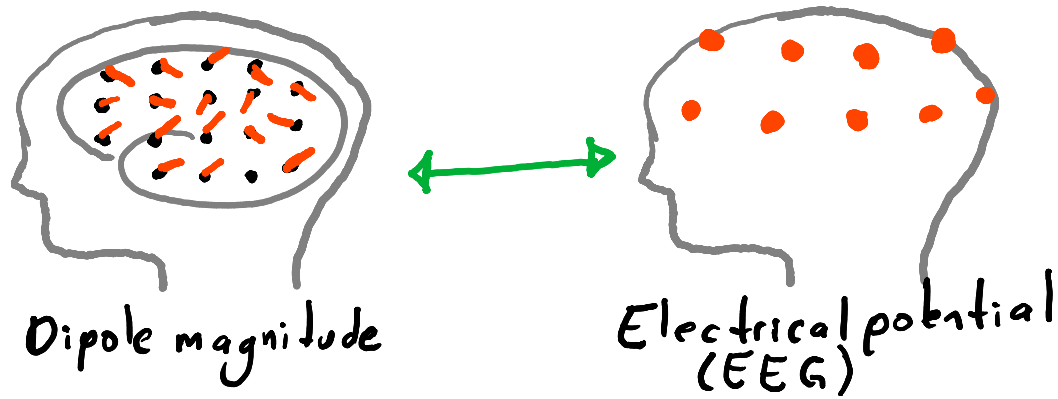
\includegraphics[width=0.75\linewidth]{./img_oldbeamer/sketch04}
\end{figure}
\end{frame}

\begin{frame}{Electrical Source Imaging Framework}
    The modeling of the dipoles starts with the \alert{current density field}, $K: \R^3 \rightarrow \R^3$, whose divergence is defined as
    \begin{equation}
        \nabla \cdot K = \lim_{G \rightarrow 0} \frac{1}{\text{vol}\ppar{G}}
        \oint_{\partial G} K\, dS
    \end{equation}
    In the presence of a single dipole with magnitude $I$, whose source is located at $\rr_{+}$ and whose sink is located at $\rr_{-}$, the divergence of th current density field reduces to
    \begin{equation}
        \nabla \cdot K(\rr) = I \delta\ppar{\rr-\rr_+} - I \delta\ppar{\rr-\rr_-}
        \label{eq:curr_density}
    \end{equation}
\end{frame}

\begin{frame}{Previous Results}
Electrical Source Imaging was used; for example, 
in
\cite{dr_pascal}.

\begin{itemize}
\item Glucose transporter type I deficiency (G1D) causes nutrient-responsive epilepsy
\item EEG was recorded for 23 hours following the monitoring
of 6 G1D subjects (ages 2-19)
\item 81 seizures (2-15 minutes) were analyzed
\item ESI was performed using sLORETA
\item ESI results were downsampled in space to the LPA40 anatomical atlas and in time to 20\% segments
\item From 20\% to 40\% of duration, significant changes of relative power (with respect to baseline) were observed to be significant on
the sensorimotor cortex and the thalamus.
\end{itemize}
\end{frame}

{
%\metroset{background=dark}
\section{Forward Problem}
}

\begin{frame}{Neuron Dipoles}
\begin{itemize}
\item A single post-synaptic potential 
acts like an electric dipole and
produces an electric scalar field, $V$. 
%This can be modeled as a single dipole.
\item Each single neuron is too small to produce a significant change. The combined action of all neurons produces a large current density field.
\item EEG electrodes are located finite set at $\sa_1, \sa_2, \dots, \sa_M$.
\item EEG measures a difference in scalar electric field, $V$,
\begin{equation}
\Y(m) = V\ppar{\sa_m} - V\ppar{\sa_\text{ref}}
\end{equation}
with $\sa_\text{ref}$ an `electrical neutral' point.
\end{itemize}
\end{frame}

\begin{frame}{Equivalent Dipoles}
\begin{itemize}
\item \alert{Key assumption:} Consider a finite set of \textbf{distributed dipoles}, which produce the same electric field observe by the EEG.
\item Location of these dipoles is known: $\dd_1, \dots, \dd_N$.
%\item `Silent activity' occurs when singular neuron dipoles don't fire coherently. It can't be observed using EEG.
\item Consider the $n$-th dipole as $\rho_n \ee_n$ with $\nnorm{\ee_n}_2=1$.
\end{itemize}
\begin{figure}
\centering
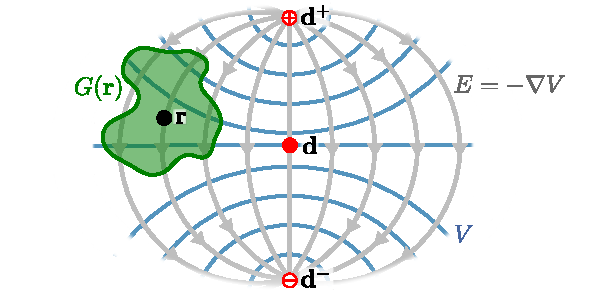
\includegraphics[width=0.45\linewidth]{./img/CurrDensField}
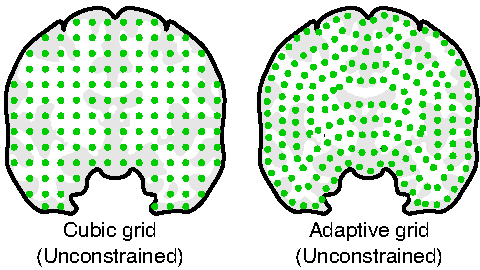
\includegraphics[width=0.45\linewidth]{./img/Pregions_pic_radial_v2}
\end{figure}
\end{frame}

\begin{frame}{Green Equation for 1 dipole + 1 sensor}
\begin{itemize}
\item Consider the $m$-th EEG sensor and the $n$-th equivalent dipole.
\item The electrical potential field, $V$, follows
\begin{equation}
\nabla \cdot\ppar{\sigma(\rr)\, \nabla V(\rr) } = 
\rho\spar{ \delta\ppar{\rr-\ee_n^+} + \delta\ppar{\rr-\ee_n^-} }
\label{eq:01}
\end{equation}
with $\sigma\ppar{\rr}$ the conductivity.
\item For the isotropic case, $\sigma\ppar{\rr}= \kappa \id$, equation \ref{eq:01} reduces to 
\begin{equation}
\kappa\, \Delta { V(\rr) } = 
\rho\spar{ \delta\ppar{\rr-\ee_n^+} + \delta\ppar{\rr-\ee_n^-} }
\label{eq:02}
\end{equation}
\end{itemize}
\end{frame}

\begin{frame}{Green Equation: Domain}
\begin{itemize}
\item We use the 4-sphere model: the domain is 4 media (brain, CSF, skull, head) with regional-constant conductivity.
\item Solutions must be regular:
%\begin{equation}
$\sigma(\bullet)\, V(\bullet) \in C^1 \ppar{\mathcal{M}_1 \cup \dots, \cup \mathcal{M}_4}$.
%\end{equation}
\item Air is non-conductive, so we use reflective boundary conditions
\begin{equation}
\kappa\, \nabla V(\rr) \cdot \mathbf{n} = 0, \text{ for } \rr\in \mathcal{M}_1.
\end{equation}
\begin{figure}
\centering
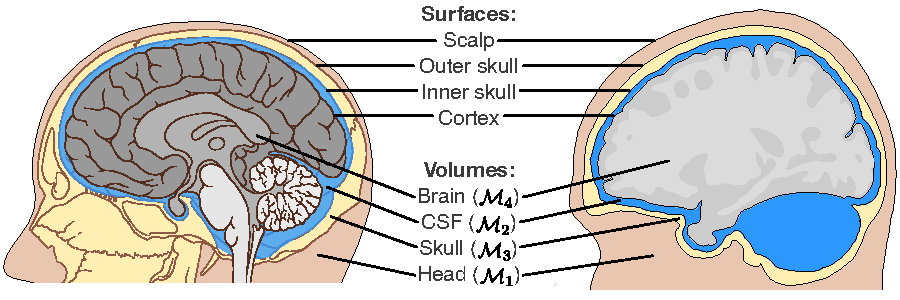
\includegraphics[width=0.8\linewidth]{./img/HeadSurfacesVolumes}
\end{figure}
\end{itemize}
\end{frame}

\begin{frame}{Green Equation for $M$ sensors + $N$ dipole}
\begin{itemize}
\item Consider $\tilde{V}_n$ the solution to 
\begin{equation}
\kappa\, \Delta { \tilde{V}_n(\rr) } = 
{ \delta\ppar{\rr-\ee_n^+} + \delta\ppar{\rr-\ee_n^-} },
\end{equation}
\item The electrical scalar field from all the equivalent dipoles, at the $m$-th sensor, is given by
\begin{equation}
V(\sa_m) = \sum_{n=1}^N \rho_n \tilde{V}_n \ppar{\sa_m}
=
\begin{bmatrix}
\tilde{V}_1 \ppar{\sa_m} &
\cdots &
\tilde{V}_N \ppar{\sa_m}
\end{bmatrix}
\begin{bmatrix}
\rho_1 \\ \vdots \\ \rho_N
\end{bmatrix}
\label{eq:stack}
\end{equation}
\end{itemize}
\end{frame}

\begin{frame}{Resulting Model}
\begin{itemize}
\item Observation from $M$ sensors can be stacked as
\begin{equation}
\begin{bmatrix}
V\ppar{\sa_1}
\\
V\ppar{\sa_2}
\\
\vdots \\
V\ppar{\sa_M}
\end{bmatrix}
=
\begin{bmatrix}
\tilde{V}_1 \ppar{\sa_1} &
\tilde{V}_2 \ppar{\sa_1} &
\cdots &
\tilde{V}_N \ppar{\sa_1} \\
\tilde{V}_1 \ppar{\sa_2} &
\tilde{V}_2 \ppar{\sa_2} &
&
\tilde{V}_N \ppar{\sa_M} \\
\vdots &  & \ddots & \vdots \\
\tilde{V}_1 \ppar{\sa_M} &
\tilde{V}_2 \ppar{\sa_M} &
\cdots &
\tilde{V}_N \ppar{\sa_M}
\end{bmatrix}
\begin{bmatrix}
\rho_1 \\ \rho_2 \\ \vdots \\ \rho_N
\end{bmatrix}
\end{equation}
\item Such equation can be summarized as
\begin{equation}
\Y = \G \SA
\end{equation}
with $\G$ referred to as the \alert{leadfield matrix}.
\item $\Y$ depends entirely on EEG data, $\G$ can be computed from anatomical data, and $\SA$ is to be found.
\end{itemize}
\end{frame}

\begin{frame}{Case of Unknown Orientation}
\begin{itemize}
%\item We may assume that dipoles at the cortex surface are orthogonal to it. This assumption is motivated by physiological observations. 
\item If the dipoles' orientation is unknown, each dipole can be projected into canonical coordinates, so
\begin{equation}
\rho_n\, \ee_n =
\rho_n^x\, \ee_n^x + \rho_n^y\, \ee_n^y + \rho_n^z\, \ee_n^z.
\end{equation}
\item To recover the original interpretation, find $\abss{\rho_n}$.
\begin{figure}
\centering
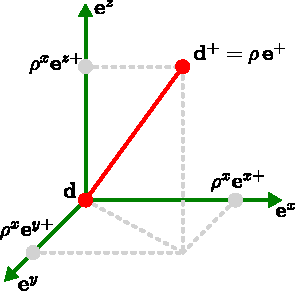
\includegraphics[width=0.4\linewidth]{./img/OrthDecomp}
\end{figure}
\end{itemize}
\end{frame}

\begin{frame}{Practical considerations}
Steps to solve the Forward Problem:
\begin{enumerate}
\item Start with anatomic MRI from subject (or template) and locations of EEG electrodes.
\item Segmentation: Identify relevant volumes.
\item Reconstruction triangulated surfaces.
\item Generate locations of distributed dipoles.
\item Solve equation \ref{eq:02} to compute $\G$.
\end{enumerate}

\end{frame}

\begin{frame}{Typical pipelin}
\begin{figure}
\centering
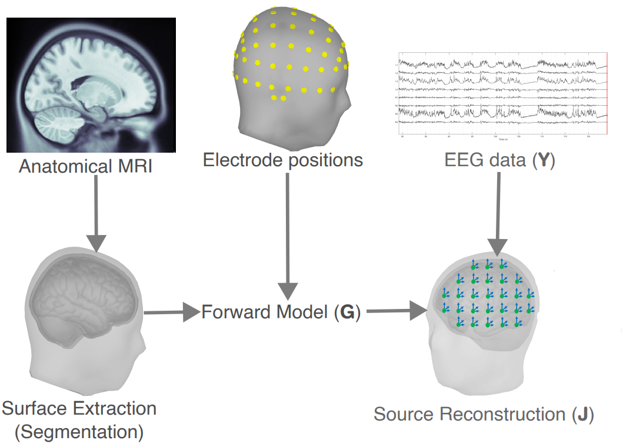
\includegraphics[width=0.7\linewidth]{./img_dev/pipeline}
\end{figure}
\end{frame}


{
%\metroset{background=dark}
\section{Literature Review}
}

\begin{frame}{Previous Methods}
%EEG source localization is old in the literature. 
This comparison is focused only on methods based on distributed dipoles. These methods, in general, can be written as
\begin{equation}
    \mathbf{M}^\delta = \mathbf{G} \mathbf{S} + \varepsilon
    \label{eq:general}
\end{equation}
%with 
\begin{itemize}
    \item[$\mathbf{M}$] Matrix of measurements, with noise
    \item[$\mathbf{S}$] Matrix of dipole magnitudes
    \item[$\mathbf{G}$] Leadfield matrix
    \item[$\varepsilon$] Matrix of additive noise at sensors
\end{itemize}

Equation \eqref{eq:general} has been used with %$\mathbf{M}$ 
data from EEG and MEG, and with 
dipoles on either known or unknown orientations
\cite{grech2008review}.

\end{frame}

\begin{frame}{Previous Methods}
Equation \eqref{eq:general} is under-determined and thus doesn't have a unique solution. One common structure is to prioritize the solutions which minimize certain penalty function
\begin{equation}
    \hat{\mathbf{S}} = \argmin_{\mathbf{S}}\, \nnorm{\G \mathbf{S}-\mathbf{M}^\delta} + \lambda\, f\ppar{\mathbf{S}}
    \label{eq:general_min}
\end{equation}
where $f$ is the penalty function, and $\lambda$ is a parameter.

\end{frame}

\begin{frame}{Previous Methods}
    For example, basic Tikhonov regularization considers $f\ppar{\mathbf{S}} = \nnorm{\mathbf{S}}_2^2$.
\begin{equation}
    \hat{\mathbf{S}}_{\text{basic}}
    =
    \G^T \ppar{\G \G^T + \lambda\, \id}^{-1} \mathbf{M}^\delta
\end{equation}

A more general Weighted Minimal Norm Estimator (WMNE) is obtained by considering
$f\ppar{\mathbf{S}} = \nnorm{W\, \mathbf{S}}_2^2$, with $W$ a positive-definite matrix. Then
\begin{equation}
    \hat{\mathbf{S}}_{\text{WMNE}}
    =
    \G^T \ppar{\G \G^T + \lambda\, W^T W}^{\dagger} \mathbf{M}^\delta
\end{equation}
\end{frame}

\begin{frame}{Previous Methods}
LORETA\cite{loreta}  considers 
$f\ppar{\mathbf{S}} = \nnorm{Q\,\overline{\G}\, \mathbf{S}}_2^2$, with $Q$ 
a Laplacian operator and $\overline{\G}$ 
a diagonal matrix
defined as
\begin{align*}
    \overline{\G}_{i,i} &= \nnorm{\G_{\bullet,i}}_2 \\
    Q_{i,j} &=
    \begin{cases}
        1 &\text{if } i=j \\
        -\frac{1}{n} &\text{if } i\in N(i) \\
        0 &\text{otherwise}
    \end{cases}
\end{align*}
with $N(i)$ a neighborhood of $i$ with $n$ grid-points.
%
\begin{equation}
    \hat{\mathbf{S}}_{\text{LORETA}}
    =
    \ppar{\overline{\G}\, Q^T\, Q\,  \overline{\G}}^{-1} \G^T
    \spar{\G \ppar{\overline{\G}\, Q^T\, Q\,  \overline{\G}}^{-1} \G^T}^{\dagger} 
    \mathbf{M}^\delta
\end{equation}
\end{frame}

\begin{frame}{Previous Methods}
sLORETA\cite{sloreta}  considers a small variant of the minimization function
\begin{equation}
    \hat{\mathbf{S}} = \argmin_{\mathbf{S}}\, \nnorm{\G \mathbf{S}-\mathbf{M}^\delta-c \mathbb{1}} + \lambda\, f\ppar{\mathbf{S}}
\end{equation}
with $f\ppar{\mathbf{S}} = \nnorm{\mathbf{S}}_2^2$ and 
$\mathbb{1}=\{1\}^{M\times 1}$.
The solution is given by
\begin{equation}
    \hat{\mathbf{S}}_{\text{sLORETA}}
    =
    \G^T H\spar{H\, \G\, \G^T H+ \lambda H}^{\dagger}
    \mathbf{M}^\delta
\end{equation}
with $H$ an averaging operator constructed as
\begin{equation*}
    H = \id - \ppar{\mathbb{1} \mathbb{1}^T}/\ppar{\mathbb{1}^T \mathbb{1}}
\end{equation*}

\end{frame}

\begin{frame}{Previous Methods}
All the mentioned methods, as well as similar others such as LAURA\cite{LAURA},  FOCUSS\cite{focuss}, among others,
can be interpreted as WMNEs 
specific
weight matrices.

In general, for autonomous\footnote{Penalization is independent of time.} WMNEs, the source estimations can be written as a filter of the observations,
\begin{equation}
    \hat{\mathbf{S}}
    =
    \mathbf{K}\,
    \mathbf{M}^\delta
\end{equation}
with $\mathbf{K}$ known as a \alert{Wiener kernel}.
\end{frame}

\begin{frame}{Previous Methods}
Some selections of the penalty function lead to solutions with desirable properties but not closed-form solutions.

For example, $f(\mathbf{S}) = \nnorm{\mathbf{S}}_1$ can be solved efficiently \cite{review_sparse}, but the solution can't be written as a Wiener Kernel.

The existence of a Wiener Kernel is desirable when the number of dipoles and time points is particularly large. This is the case for long-term monitoring of spontaneous activity.
\end{frame}





{
%\metroset{background=dark}
\section{Numerical Experiments}
}

\begin{frame}{A}

\end{frame}

{
%\metroset{background=dark}
\section{Proposed Model}
}

\begin{frame}{Previous Methods for Multimodal Data}
One big conceptual challenge for multimodal data integration is to model the interaction of the underlying physical phenomena. 
%
Focusing only on unilateral interactions results in asymmetric data integration.

\alert{Asymmetric data fusion} is the extraction of some parameters from one modality, which then are used to further the analysis of the other modality.

Some of the parameters extracted include:
\begin{itemize}
    \item Correlation networks
    \item Statistical Parametric Maps (SPM)
    \item Hidden activation variables \cite{fire}
\end{itemize}

\end{frame}

\begin{frame}{Dataset Framework}
The goal is to study the effects of
ischemic stroke of the Middle Cerebral Artery in an animal
model. 
Said lesion is induced.

Electro Corticogram (ECoG) is placed. Recordings start before the lesion and stop 2 hours after it.

In the post-mortem, the brain is stained with
triphenyl-tetrazolium (TTC)
to identify tissues damaged by hypoxia. This information is referred to as \alert{symptoms}.

\begin{figure}
\centering
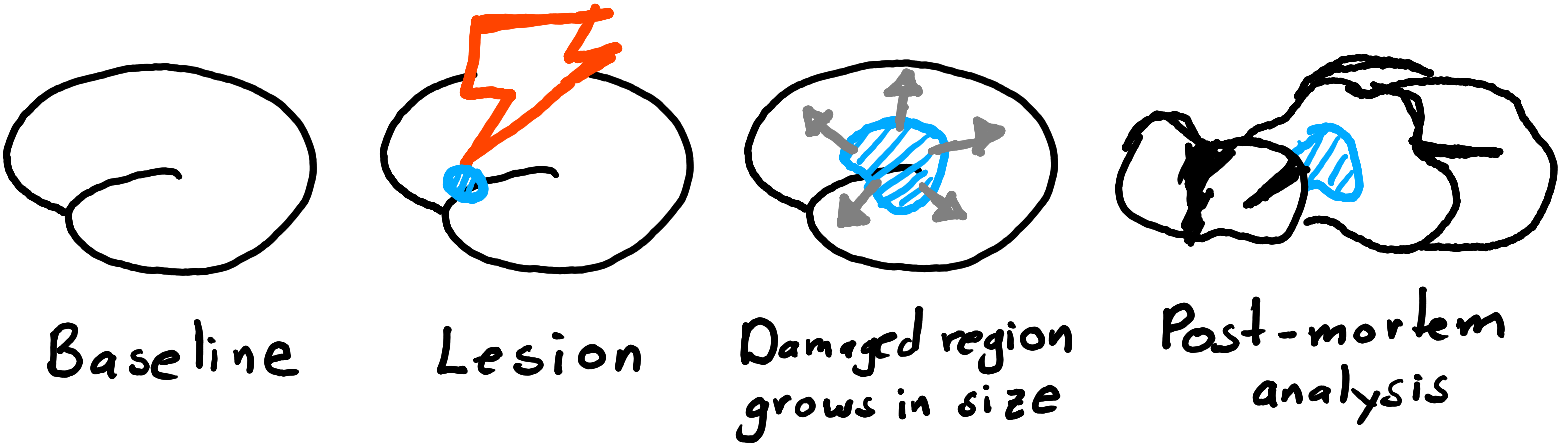
\includegraphics[width=0.8\linewidth]{./img_oldbeamer/sketch01_v2}
\end{figure}
\end{frame}

\begin{frame}{Proposed Work}
The proposed innovation is to use the information from {symptoms} to enhance the results of ESI.
%
A posterior analysis of the results of this ESI may help identify the damaged zone as it evolves over time.

This new model considers two phases:
\begin{enumerate}
    \item Static symptoms (finished, reporting now).
    \item Time-changing symptoms.
\end{enumerate}
\end{frame}





\begin{frame}{Observed symptoms}
The post-mortem observations, referred to as \alert{symptoms}, are registered against a template brain. 

This information is used to label the dipoles in the grid using
${S\in \sset{0,1}^{N\times 1}}$, so that $S_n = 1$ if the $n$-th dipole is located on a region where symptoms were observed.

\begin{figure}
\centering
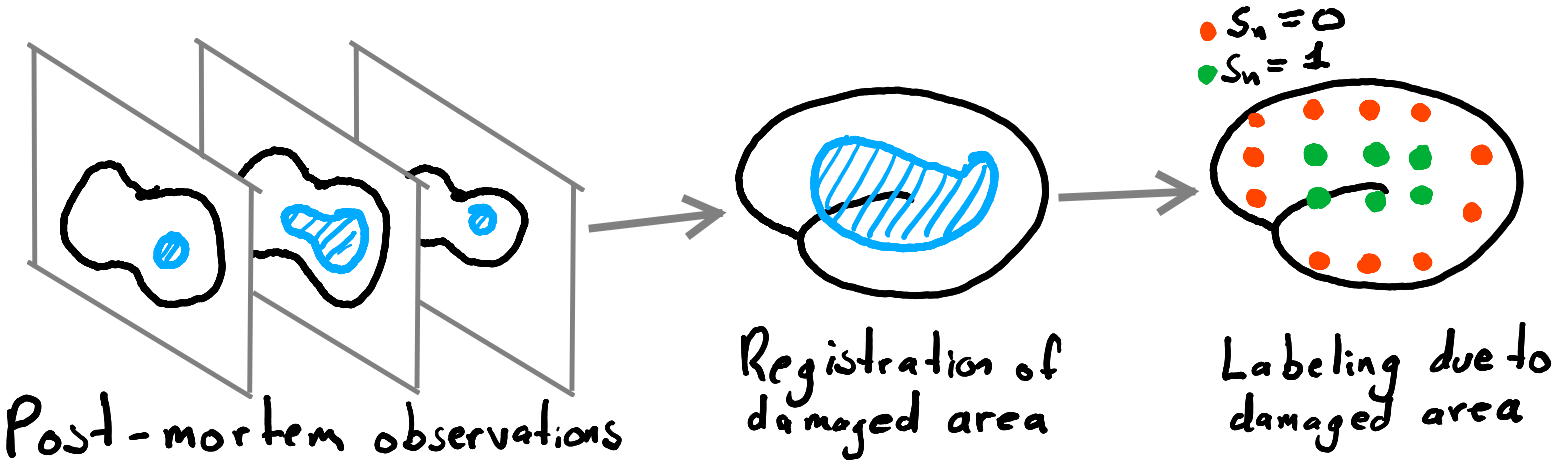
\includegraphics[width=0.8\linewidth]{./img_oldbeamer/sketch02_v2}
\end{figure}

\end{frame}



\begin{frame}{Effect of Observed Symptoms}
The relation between symptoms and current density ($\J$) is modeled by adjusting the expected value of the latter based on the symptoms label ($S$).
\begin{equation}
    E\spar{\J_{t,n}} = 
    \begin{cases}
        \U_{t,k} & \text{if } S_n=1 \text{ and } n\in R_k \\
        0 & \text{if } S_n=0
    \end{cases}
\end{equation}

This formulation is equivalent to stating that
\begin{equation}
    \J = \text{diag}\ppar{S} L \U + \N
\end{equation}
where $\mathbf{U}\in \R^{K\times T}$ and $\mathbf{N}\in \R^{N\times T}$ are independent and satisfy
\begin{equation}
    \text{Var}\ppar{\N_{t,n}} \ll \text{Var}\ppar{\U_{t,k}}.
\end{equation}
\end{frame}

\begin{frame}{Distributions from the model}
The proposed model is driven by the following equations
\begin{align}
    \Y &= \G \J + \varepsilon \\
    \J &=  L_S \U + \N
\end{align}
where $\Y, \G$ and $L_S = \text{diag}\ppar{S} L$ are given, and
\begin{align}
    \varepsilon_t &\sim  \norm\ppar{0, \sigma^2 \id } \\
    \N_t &\sim  
    \norm\ppar{0, \gamma_0^2 \id } \\
    \U_t &\sim  
    \norm\ppar{0, \gamma_1^2 \id } 
\end{align}
with $\gamma_0^2 \ll \gamma_1^2$.
\end{frame}



\begin{frame}{Maximum A Posteriori (MAP) estimator}
The estimator is derived from maximizing the a posteriori probability,
\begin{align}
    \ppar{ \hat{\U}, \hat{\N} } &=
    \argmax_{\U, \N }\,
    \log P\ppar{\ppar{ {\U}, {\N} } \Big| {\Y; \gamma_0, \gamma_2} }
\end{align}
which derives into the following error function
\begin{align}
    F\ppar{ {\U}, {\N};  \gamma_0, \gamma_1} &=
    \frac{1}{2\sigma^2}
    \nnorm{\G L_S \U + \G \N - \Y}_F^2
    \nonumber \\
    &\phantom{=}
    +
    \frac{1}{2\gamma_0^2} \nnorm{\N}_F^2
    +
    \frac{1}{2\gamma_1^2} \nnorm{L_S \U}_F^2
\end{align}
\end{frame}

\begin{frame}{Maximum A Posteriori (MAP) estimator}
    The iterative minimization of the error function can be interpreted as a multi-scale iterative correction
    \begin{align}
        \hat{\N}^{(i+1)} &= \argmin_{\N} F\ppar{\U^{(i)},\N; \gamma_0, \gamma_1}
        \\
        \hat{\U}^{(i+1)} &= \argmin_{\U} F\ppar{\U,\N^{(i)}; \gamma_0, \gamma_1}
    \end{align}
    These steps have the following closed-form
    \begin{align}
        \hat{\N}^{(i+1)} &=
        \hat{\N}^{(i)}
        -
        \G^T \spar{\G \G^T + \frac{\gamma_0^2}{\sigma^2} \id}^{-1} L_S \ppar{\hat{\U}^{(i)}-\hat{\U}^{(i-1)} }
        \\
        \hat{\U}^{(i+1)} &=
        \hat{\U}^{(i)}
        -
        L_S^T \G^T \spar{\G L_S L_S^T \G^T + \frac{\gamma_1^2}{\sigma^2} \id}^{-1} \ppar{\hat{\N}^{(i)}-\hat{\N}^{(i-1)} }
    \end{align}
\end{frame}

{
%\metroset{background=dark}
\subsection{Derivation of the Estimator}
}

\begin{frame}
\begin{align*}
    \ppar{ \hat{\U}, \hat{\N} } &=
    \argmax_{\U, \N }\,
    \log P\ppar{\ppar{ {\U}, {\N} } \Big| {\Y; \gamma_0, \gamma_2} }
    \\
    &=
    \argmax_{\U, \N }\, \sum_{t=1}^T 
    \log P\ppar{\ppar{ {\U_t}, {\N_t} } \Big| {\Y_t; \gamma_0, \gamma_2} }
    \\
    &=
    \argmax_{\U, \N }\, \sum_{t=1}^T  \left[
    \log P\ppar{{ \Y_t } \Big| { \ppar{\U_t, \N_t}  ; \gamma_0, \gamma_2} }
    \right.
    \\
    &\phantom{=}
    \left.
    +
    P\ppar{{ {\U_t}  ; \gamma_0, \gamma_2} }
    +
    P\ppar{{ {\N_t}  ; \gamma_0, \gamma_2} }
    \right]
    \\
    &=
    \argmax_{\U, \N }\, \sum_{t=1}^T  \left[
    -\frac{1}{2\sigma^2}
    \nnorm{\G L_S \U_t + \G \N_t - \Y_t}_2^2
    \right.
    \\
    &\phantom{=}
    \left.
    -
    \frac{1}{2\gamma_0^2} \nnorm{\N_t}_2^2
    -
    \frac{1}{2\gamma_1^2} \nnorm{L_S \U_t}_2^2
    \right]
\end{align*}
\end{frame}

\begin{frame}
\begin{align*}
\ppar{ \hat{\U}, \hat{\N} } 
&=
    \argmax_{\U, \N }\, \sum_{t=1}^T  \left[
    -\frac{1}{2\sigma^2}
    \nnorm{\G L_S \U_t + \G \N_t - \Y_t}_2^2
    \right.
    \\
    &\phantom{=}
    \left.
    -
    \frac{1}{2\gamma_0^2} \nnorm{\N_t}_2^2
    -
    \frac{1}{2\gamma_1^2} \nnorm{L_S \U_t}_2^2
    \right]
    \\
    &=
    \argmax_{\U, \N }\, \left[
    -\frac{1}{2\sigma^2}
    \nnorm{\G L_S \U + \G \N - \Y}_F^2
    \right.
    \\
    &\phantom{=}
    \left.
    -
    \frac{1}{2\gamma_0^2} \nnorm{\N}_F^2
    -
    \frac{1}{2\gamma_1^2} \nnorm{L_S \U}_F^2
    \right]
\end{align*}
\end{frame}

\begin{frame}
This derives into the following error function
\begin{align*}
    F\ppar{ {\U}, {\N};  \gamma_0, \gamma_1} &=
    \frac{1}{2\sigma^2}
    \nnorm{\G L_S \U + \G \N - \Y}_F^2
    \nonumber \\
    &\phantom{=}
    +
    \frac{1}{2\gamma_0^2} \nnorm{\N}_F^2
    +
    \frac{1}{2\gamma_1^2} \nnorm{L_S \U}_F^2
\end{align*}
So that
\begin{align*}
\ppar{ \hat{\U}, \hat{\N} } 
&=
    \argmin_{\U, \N }\, F\ppar{ {\U}, {\N};  \gamma_0, \gamma_1}
\end{align*}
Notice that the function is convex in both $\U$ and $\N$, and thus it can be minimized iteratively over it's arguments,
    \begin{align*}
        \hat{\N}^{(i+1)} &= \argmin_{\N} F\ppar{\U^{(i)},\N; \gamma_0, \gamma_1}
        \\
        \hat{\U}^{(i+1)} &= \argmin_{\U} F\ppar{\U,\N^{(i)}; \gamma_0, \gamma_1}
    \end{align*}
\end{frame}

\begin{frame}
Minimization is carried away via Lagrange multipliers with the constraint $\G L_S \U + \G \N - \Y=0$.
\begin{align*}
    \hat{\N}^{(i+1)} &= \argmin_{\N}  F\ppar{\U^{(i)},\N; \gamma_0, \gamma_1}
    \\
    &\phantom{=}
    \quad \quad
    \text{st} \quad \quad
    \G L_S \U^{(i)} + \G \N - \Y=0
\end{align*}
This leads to the Lagrangian function
\begin{align*}
    \mathscr{L}_\N \ppar{\N, \lambda; \U^{(i)}, \gamma_0}
    &=
    \frac{1}{2\sigma^2}
    \nnorm{\G L_S \U^{(i)} + \G \N - \Y}_F^2
    +
    \frac{1}{2\gamma_0^2} \nnorm{\N}_F^2
    \\
    &\phantom{=}
    +\lambda^T\ppar{\G L_S \U^{(i)} + \G \N - \Y}
\end{align*}
\end{frame}

\begin{frame}
\begin{align*}
\frac{\partial}{\partial \N}
\mathscr{L}_\N \ppar{\N, \lambda; \U^{(i)}, \gamma_0}
    &=
    \frac{1}{\sigma^2}
    \G^T
    \ppar{\G L_S \U^{(i)} + \G \N - \Y}
    \\
    &\phantom{=}
    +
    \frac{1}{\gamma_0^2} {\N}
    +
    \G^T \lambda
    \\
    \frac{\partial}{\partial \lambda} 
    \mathscr{L}_\N \ppar{\N, \lambda; \U^{(i)}, \gamma_1}
    &=
    \G L_S \U^{(i)} + \G \N - \Y
\end{align*}
By setting $\frac{\partial}{\partial \N} \mathscr{L}_\N = 0$ and 
$\frac{\partial}{\partial \lambda} \mathscr{L}_\N = 0$, it arises the conditions
\begin{align*}
    {\frac{1}{\gamma_0^2} { \N}
    +
    \G^T \lambda} &= 0
    \\
    \G \N 
    &= \Y - \G L_S \U^{(i)} 
\end{align*}
\end{frame}

\begin{frame}
\begin{align*}
&&
{\frac{1}{\gamma_0^2} { \N}
    +
    \G^T \lambda} &= 0
\\
\Rightarrow
&&
\N &= -\gamma_0^2 \G^T \lambda
\\
\Rightarrow
&&
-\gamma_0^2 \G \G^T \lambda
&=
\Y - \G L_S \U^{(i)} 
\\
\Rightarrow
&&
\lambda &=
-\frac{1}{\gamma_0^2} \spar{\G \G^T+ \frac{\gamma_0^2}{\sigma^2}^{-1}}^{-1} \ppar{\Y - \G L_S \U^{(i)} }
\\
\Rightarrow
&&
\N &=
\G^T \spar{\G \G^T+ \frac{\gamma_0^2}{\sigma^2}^{-1}} \ppar{\Y - \G L_S \U^{(i)} }
\end{align*}
Thus, concluding the following
\begin{align*}
\N^{(i+1)} &=
\G^T \spar{\G \G^T+ \frac{\gamma_0^2}{\sigma^2}^{-1}} \ppar{\Y - \G L_S \U^{(i)} }
\end{align*}
\end{frame}

\begin{frame}{Maximum A Posteriori (MAP) estimator}
For the iterative step, consider the following,
\begin{align*}
\N^{(i+1)} &=
\G^T \spar{\G \G^T+ \frac{\gamma_0^2}{\sigma^2}^{-1}} \ppar{\Y - \G L_S \U^{(i)} }
\\
\N^{(i)} &=
\G^T \spar{\G \G^T+ \frac{\gamma_0^2}{\sigma^2}^{-1}} \ppar{\Y - \G L_S \U^{(i-1)} }
\\
\Rightarrow
\N^{(i+1)}-\N^{(i)} &=
\G^T \spar{\G \G^T+ \frac{\gamma_0^2}{\sigma^2}^{-1}} \G L_S \ppar{ \U^{(i)}-\U^{(i-1)} }
\end{align*}
\end{frame}

\begin{frame}{Maximum A Posteriori (MAP) estimator [repeated slide]}
    The iterative minimization of the error function can be interpreted as a multi-scale iterative correction
    \begin{align}
        \hat{\N}^{(i+1)} &= \argmin_{\N} F\ppar{\U^{(i)},\N; \gamma_0, \gamma_1}
        \\
        \hat{\U}^{(i+1)} &= \argmin_{\U} F\ppar{\U,\N^{(i)}; \gamma_0, \gamma_1}
    \end{align}
    These steps have the following closed-form
    \begin{align}
        \hat{\N}^{(i+1)} &=
        \hat{\N}^{(i)}
        -
        \G^T \spar{\G \G^T + \frac{\gamma_0^2}{\sigma^2} \id}^{-1} L_S \ppar{\hat{\U}^{(i)}-\hat{\U}^{(i-1)} }
        \\
        \hat{\U}^{(i+1)} &=
        \hat{\U}^{(i)}
        -
        L_S^T \G^T \spar{\G L_S L_S^T \G^T + \frac{\gamma_1^2}{\sigma^2} \id}^{-1} \ppar{\hat{\N}^{(i)}-\hat{\N}^{(i-1)} }
    \end{align}
\end{frame}



{
%\metroset{background=dark}
\subsection{Numerical Experiments}
}

\begin{frame}{Numerical experiments}
Synthetic data is simulated with one source at a known location at different SNR levels. 
\begin{figure}
\centering
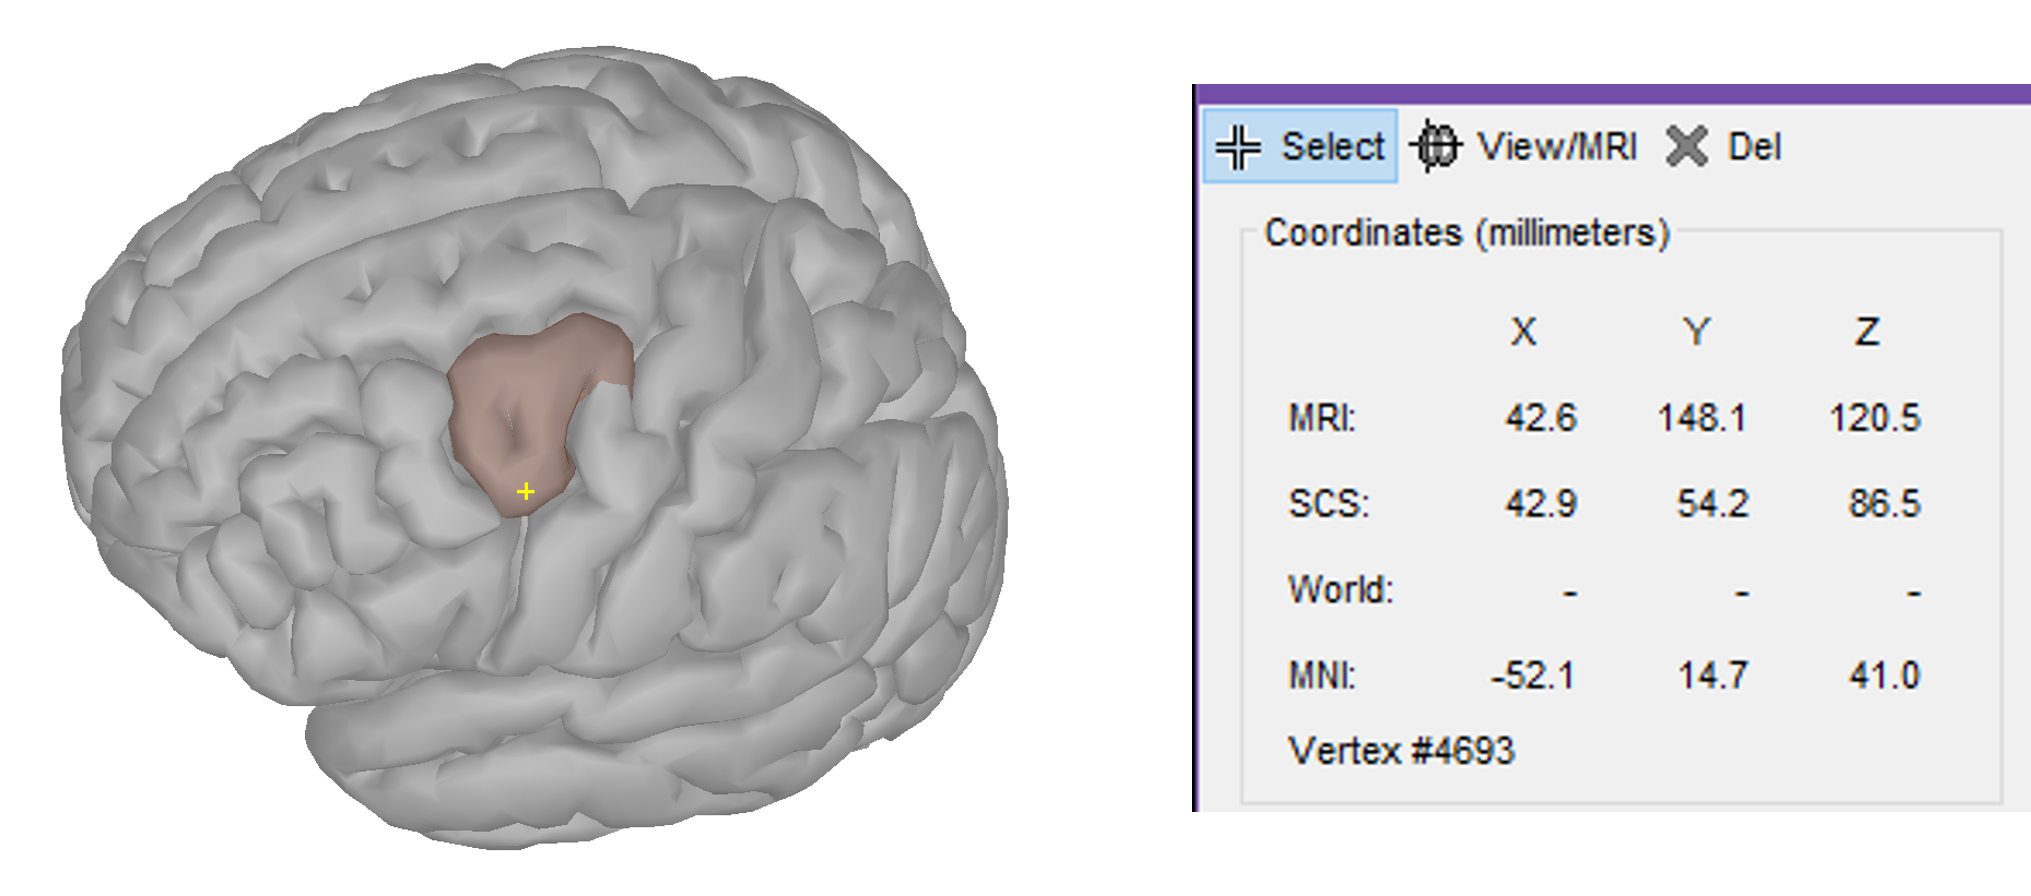
\includegraphics[width=0.8\linewidth]{./img_oldbeamer/protocol1}
\end{figure}
\end{frame}

\begin{frame}{SNR = 10}
Left to right: Classic Tikhonov, sLORETA, proposed method
\begin{figure}
\centering
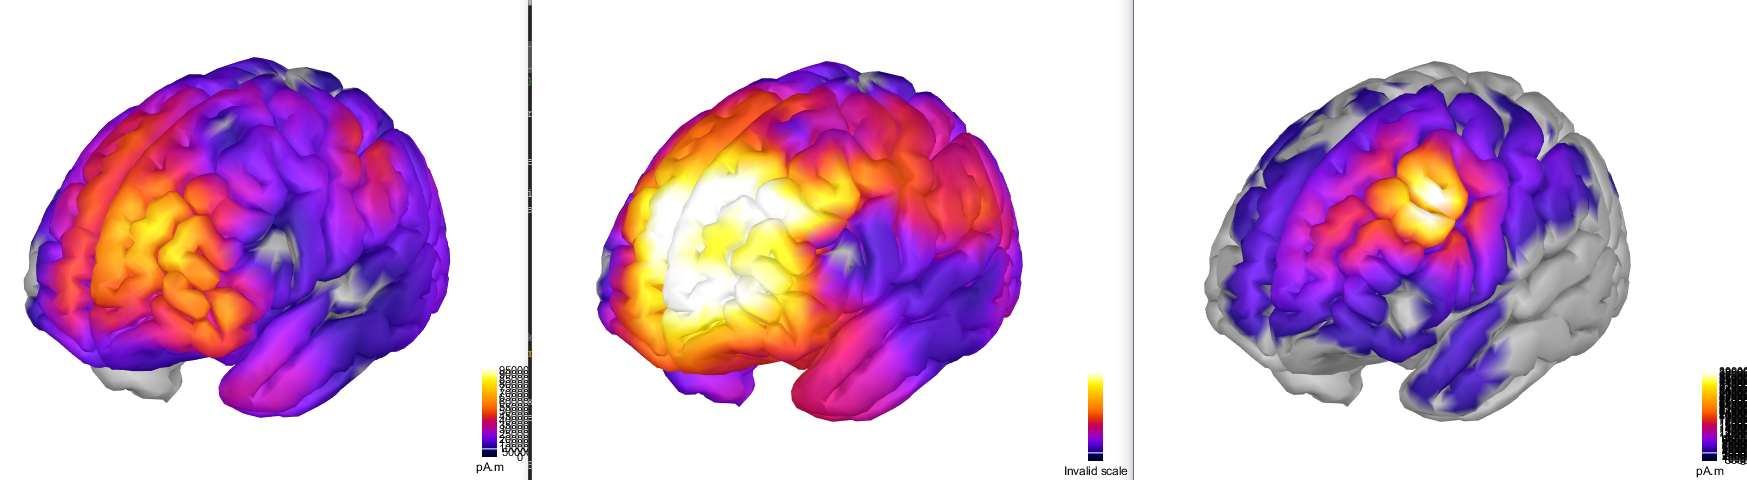
\includegraphics[width=1\linewidth]{./img_oldbeamer/comparison1}
\end{figure}
\end{frame}


{
%\metroset{background=dark}
\subsection{Future Work}
}

\begin{frame}{Future work}
\begin{itemize}
    \item The implemented method expands over previous methods for ESI by incorporating information from binary symptoms observed in the brain.
    \item As a first phase, these binary symptoms are assumed to be static over time. However, there is enough physiological information to claim that the damaged area grows over time.
    \item This time-changing damaged area can be incorporated into the model by including a time-changing vector of symptoms, ${S\in \sset{0,1}^{N\times T}}$.
\end{itemize}
\end{frame}

\begin{frame}{Future work}
The following equations drive the proposed new model
\begin{align}
    \Y &= \G \J + \varepsilon \\
    \J_t &=  L_{S_t} \U_t + \N_t
\end{align}
where $\Y, \G$ and $L_{S_t} = \text{diag}\ppar{S_t} L$ are given, and
\begin{align}
    \varepsilon_t &\sim  \norm\ppar{0, \sigma^2 \id } \\
    \N_t &\sim  
    \norm\ppar{0, \gamma_0^2 \id } \\
    \U_t &\sim  
    \norm\ppar{0, \gamma_1^2 \id } 
\end{align}
with $\gamma_0^2 \ll \gamma_1^2$.
\end{frame}

\begin{frame}{Thanks for your attention}

\end{frame}

%{
%%\metroset{background=dark}
%\section{Bibliography}
%}

%\begin{frame}[allowframebreaks]
%        \frametitle{References}
%\bibliographystyle{abbrv} % We choose the "plain" reference style
%%\bibliography{./refs_old} % Entries are in the refs.bib file
%\bibliography{./refs} % Entries are in the refs.bib file
%\end{frame}

\begin{frame}[allowframebreaks]
  \frametitle{References}
  \printbibliography
\end{frame}

\end{document}